\documentclass{article}
\usepackage[utf8]{inputenc}
\usepackage{natbib}
\usepackage{hyperref}
\usepackage{graphicx}
\usepackage{subcaption}
\usepackage{amssymb,amsmath,amsthm}
\usepackage{xcolor}
\usepackage{xspace}
\usepackage[nameinlink,capitalize]{cleveref}
\usepackage{cleveref}
\usepackage{geometry}
\usepackage{pdflscape}
\usepackage{epstopdf} %converting to PDF
\newcommand{\Rnum}{\mathcal{R}_0}
\title{Fast and less-accurate coronavirus tests vs slow and more-accurate coronavirus tests }
\author{Ali Gharouni}
\date{December 2020}

\newcommand{\comment}{\showcomment}
\newcommand{\showcomment}[3]{\textcolor{#1}{\textbf{[#2: }\textsl{#3}\textbf{]}}}
\newcommand{\nocomment}[3]{}

\newcommand{\fady}[1]{\comment{cyan}{Lin}{#1}}
\newcommand{\ali}[1]{\comment{magenta}{Ali}{#1}}
\newcommand{\todo}[1]{\comment{red}{TODO}{#1}}

\theoremstyle{definition} % amsthm only
\newtheorem{proposition}{Proposition}
\newtheorem{note}{Note}
\newtheorem{theorem}{Theorem}

\bibliographystyle{apalike}

\begin{document}
\maketitle
% %%%%%%%%%%%%%%%%%%%%%%%%%%%%%%%%%%%%%%%%%%%%%%%%%%%%%%%%%%%
\section{Introduction}
% %%%%%%%%%%%%%%%%%%%%%%%%%%%%%%%%%%%%%%%%%%%%%%%%%%%%%%%%%%%
\begin{itemize}
  \item Say something about current testing strategies and methods
  \item reporting procedure
  \item waiting time
\end{itemize}



{\bf current testing strategies, methods and accuracy;}

- The influence of testing processes on the epidemic dynamics through isolation has been studied here.
- Testing methods;
    - The accuracy of the test is subject to the sampling method. Also, detection rates in any sample type may vary from patient to patient but also may change over the course of the infection \citep{patel2020report}.
    - include Nasopharyngeal swab, sputum, saliva, stools, or a combination. There is an ongoing research to identify the best testing method.
    - For an overview of different methods of testing and accuracy see \cite{machado2021main}.
    - Up to now the sensitivity of the available test for diagnosing COVID-19 is between 70\% to 90\% \citep{woloshin2020false.}.


Here The ``sensitivity'' of a test is defined as the ability of a test to produce a positive result for a true infected individual. On the other hand, ``specificity'' is the ability of a test to correctly produce the negative result for an uninfected individual.  








old stff from the SIR model:
One of the main challenges in understanding COVID-19 dynamics is to unravel information available from data. The daily case count is a highly accessible form of data where observations are driven by two clusters of processes: (i) epidemic processes and (ii) testing processes. The challenge is then to separate these processes and understand how they interact. Simple mathematical models have a long history in providing useful insights facing with real epidemiological challenges \citep{ross1911prevention} [maybe add influenza work, ideas?]. We developed a model that incorporates mechanistic processes of epidemic processes and testing. We used the model to study the potential effect of testing strategies on disease dynamics.

the scale of testing, isolation and quarantine during the CIVID-19 pandemic marks one of the greatest global experiences in 21st century.
% %%%%%%%%%%%%%%%%%%%%%%%%%%%%%%%%%%%%%%%%%%%%%%%%%%%%%%%%%%%
\section{Analysis}
% %%%%%%%%%%%%%%%%%%%%%%%%%%%%%%%%%%%%%%%%%%%%%%%%%%%%%%%%%%%

% %%%%%%%%%%%%%%%%
\subsection{DFE}

Let $\bar{N} =\frac{N_0}{\omega_2 \theta_s \rho_s \alpha + 
\omega_1 \omega_2 (\alpha+\theta_s) + \omega_1 \theta_s (1-\rho_s) \alpha}$, then the DFE is 
$$E_0=(S_u^*,S_w^*,S_n^*,S_p^*,0,0,0,0,0,0,0,0,0),$$ where
$S_u^*= \alpha \omega_1 \omega_2 \bar{N}$,
$S_w^*= \theta_s \omega_1 \omega_2 \bar{N}$, 
$S_n^*=\theta_s \rho_s \alpha \omega_2 \bar{N} $, and
$S_p^*= \theta_s(1-\rho_s)\alpha \omega_1 \bar{N}$.

Note the DFE calculation is carried out by setting the infected and recovered state variables to zero, i.e., $I_z=R_z=0$ , setting $S_u+S_w+S_n+S_p=N_0$, and solving the system $dS_u/dt=0, dS_w/dt=0, dS_n/dt=0,$ and $dS_p/dt=0$ for $S_u, S_w, S_n,$ and $S_p$. 

\todo{Find $\Rnum$}.



\begin{figure}[!h] 
\begin{center} 
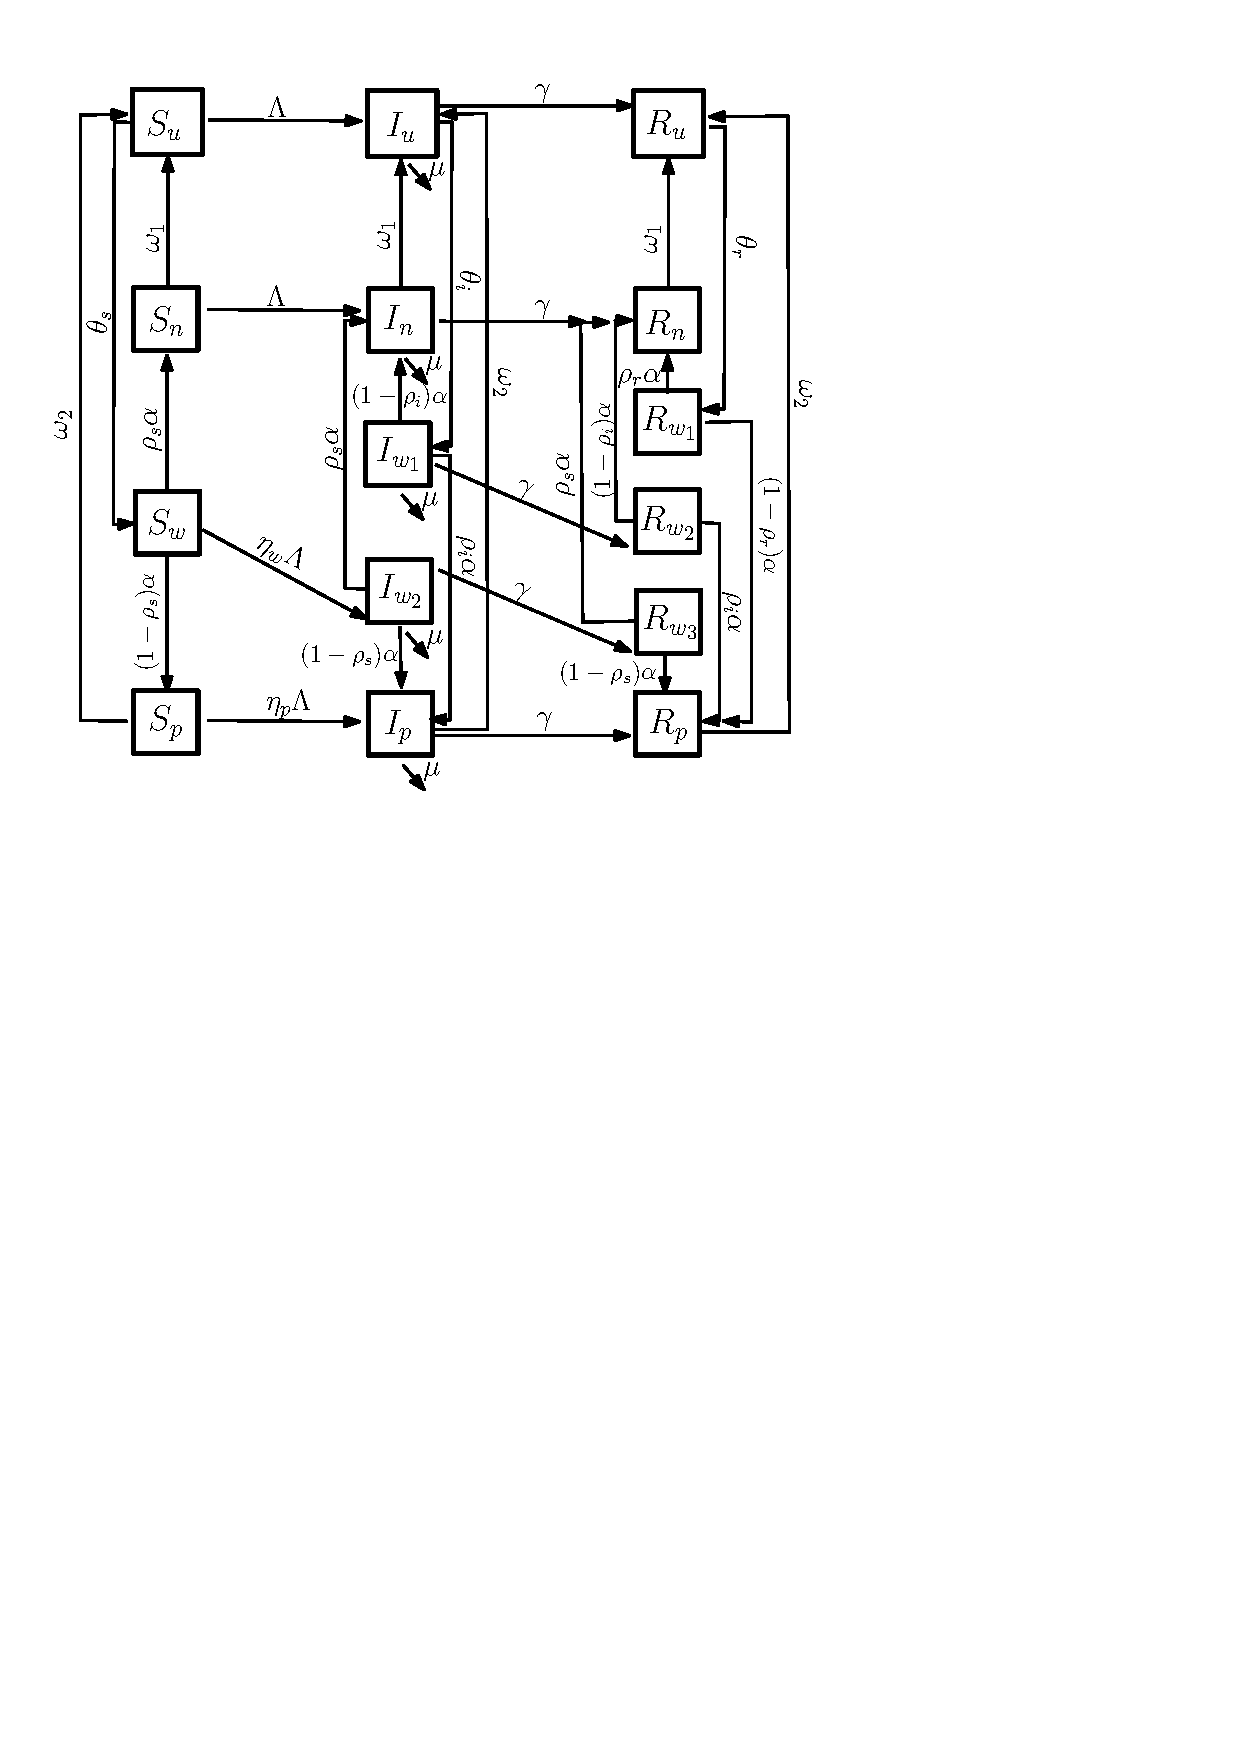
\includegraphics[scale=1]{../pix/flowchart2}
\caption{\small Flowchart of the SIR (Susceptible-Infectious-Recovered) model, \crefrange{eq1}{eq12}. For the description of the parameters see \cref{tab:params}.
\label{fig:flowchart}}
\end{center} 
\end{figure}







% %%%%%%%
\bibliography{../../SIRmodel/SIRlibrary.bib}

\end{document}
